\subsection{Simulation in Restaurant Setup}
One challenge with computing Optical Flow on simulated frames is that due to the lack of texture, it might become unstable during frames where there is zero or low level of motion in the scene. To fix this we have to preprocess the frames with a simple subtraction operator between the consecutive frames and estimate the total motion before passing the image to the optical-flow deep network.

\subsection{Why restaurants?}
\noindent
%\hl{Todo:} to read the literature and review

In fact, robots have been already deployed in restaurants and thousands of them are in place. This type of situation usually contains a certain number of people: clients, waiters, ... . And the people are part of interaction scenarios with the robot(s). The clients might be new to this place and new to facing the robot in this restaurant, which means they wouldn't have a clear idea of the robot's behavior. 


% \begin{figure}
%     \centering
%     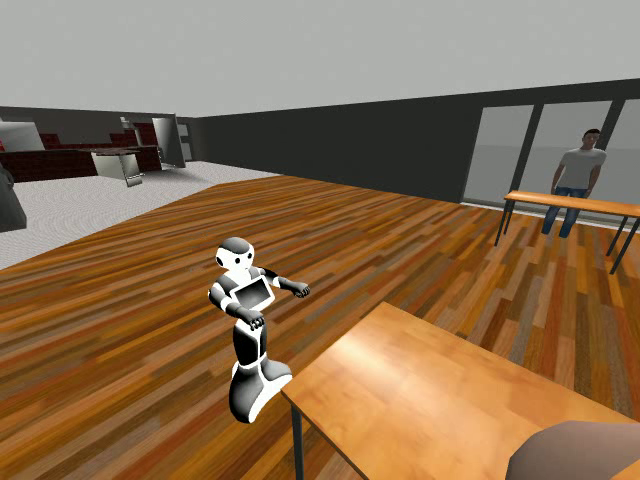
\includegraphics[width=0.4\textwidth]{figs/legibot-pepper-restaurant.png}
%     \caption{Pepper in Restaurant (Simulation)}
%     \label{fig:enter-label}
% \end{figure}

\subsection{Experiments with Real Robot}

% \begin{figure}
%     \centering
%     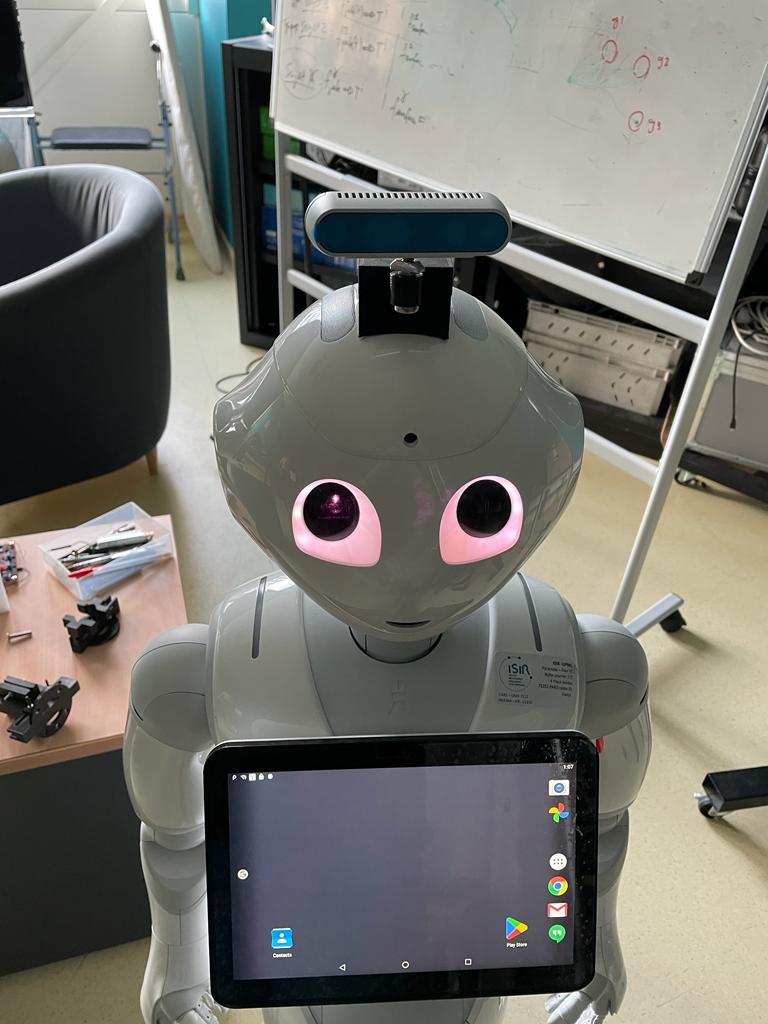
\includegraphics[width=0.3\textwidth]{figs/pepper-modified.jpeg}
%     \caption{Modified Pepper Robot}
%     \label{fig:enter-label}
% \end{figure}


\subsection{User Study}